%----------------------------------------------------------------------------------------
%   Доорх хэсгийг өөрчлөх шаардлагагүй
%----------------------------------------------------------------------------------------
%!TEX TS-program = xelatex
%!TEX encoding = UTF-8 Unicode
\documentclass[12pt,A4]{report}

\usepackage{fontspec,xltxtra,xunicode}
\setmainfont[Ligatures=TeX]{Times New Roman}
\setsansfont{Arial}

% \usepackage[utf8x]{inputenc}
% \usepackage[mongolian]{babel}
%\usepackage{natbib}
\usepackage{geometry}
%\usepackage{fancyheadings} fancyheadings is obsolete: replaced by fancyhdr. JL
\usepackage{fancyhdr}
\usepackage{float}
\usepackage{afterpage}
\usepackage{graphicx}
\usepackage{amsmath,amssymb,amsbsy}
\usepackage{dcolumn,array}
\usepackage{tocloft}
\usepackage{dics}
\usepackage{nomencl}
\usepackage{upgreek}
\newcommand{\argmin}{\arg\!\min}
\usepackage{mathtools}
\usepackage[hidelinks]{hyperref}
\usepackage{bookmark}

\usepackage{algorithm}
\usepackage{algpseudocode}

\usepackage{listings}
\DeclarePairedDelimiter\abs{\lvert}{\rvert}%
\makeatletter
\usepackage{caption}
\captionsetup[table]{belowskip=0.5pt}
\usepackage{subfiles}

\usepackage{listings}
\renewcommand{\lstlistingname}{Код}
\renewcommand{\lstlistlistingname}{\lstlistingname ын жагсаалт}

\usepackage{color}
\definecolor{codegreen}{rgb}{0,0.6,0}
\definecolor{codegray}{rgb}{0.5,0.5,0.5}
\definecolor{codepurple}{rgb}{0.58,0,0.82}
\definecolor{backcolour}{rgb}{0.99,0.99,0.99}
\definecolor{darkgray}{rgb}{0.99,0.103,0.105}
\definecolor{purple}{rgb}{0.128,0,0.128}
 
\lstdefinestyle{mystyle}{
    basicstyle=\ttfamily\small,
    backgroundcolor=\color{backcolour},   
    commentstyle=\color{codegreen},
    keywordstyle=\color{magenta},
    numberstyle=\tiny\color{codegray},
    stringstyle=\color{codepurple},
    %basicstyle=\footnotesize,
    breakatwhitespace=false,         
    breaklines=true,                 
    captionpos=b,                    
    keepspaces=false,                 
    numbers=left,                    
    numbersep=10pt,                  
    showspaces=false,                
    showstringspaces=true,
    showtabs=false,                  
    tabsize=2
}
 
 %define Javascript language
\lstdefinelanguage{JavaScript}{
keywords={typeof, new, true, false, catch, function, return, null, catch, switch, var, if, in, while, do, else, case, break},
keywordstyle=\color{blue}\bfseries,
ndkeywords={class, export, boolean, throw, implements, import, this},
ndkeywordstyle=\color{darkgray}\bfseries,
identifierstyle=\color{black},
sensitive=false,
comment=[l]{//},
morecomment=[s]{/*}{*/},
commentstyle=\color{purple}\ttfamily,
stringstyle=\color{red}\ttfamily,
morestring=[b]',
morestring=[b]"
}
 
\lstset{
language=JavaScript,
extendedchars=true,
basicstyle=\footnotesize\ttfamily,
showstringspaces=false,
showspaces=false,
numbers=left,
numberstyle=\footnotesize,
numbersep=9pt,
tabsize=2,
breaklines=true,
showtabs=false,
captionpos=b
}
 
\lstset{style=mystyle, label=DescriptiveLabel} 


\let\oldabs\abs
\def\abs{\@ifstar{\oldabs}{\oldabs*}}
\makenomenclature
\begin{document}


%----------------------------------------------------------------------------------------
%   Өөрийн мэдээллээ оруулах хэсэг
%----------------------------------------------------------------------------------------

% Дипломийн ажлын сэдэв
\title{Веб фронт-энд хөгжүүлэлт}
% Дипломын ажлын англи нэр
\titleEng{Web front-end developing}
% Өөрийн овог нэрийг бүтнээр нь бичнэ
\author{Батбаярын Бат-Өлзий}
% Өөрийн овгийн эхний үсэг нэрээ бичнэ
\authorShort{Б. Бат-Өлзий}
% Удирдагчийн зэрэг цол овгийн эхний үсэг нэр
\supervisor{С. Дөлмандах}
% Хамтарсан удирдагчийн зэрэг цол овгийн эхний үсэг нэр
\cosupervisor{Н. Оюун-Эрдэнэ}

% СиСи дугаар 
\sisiId{18B1NUM3474}
% Их сургуулийн нэр
\university{МОНГОЛ УЛСЫН ИХ СУРГУУЛЬ}
% Бүрэлдэхүүн сургуулийн нэр
\faculty{ХЭРЭГЛЭЭНИЙ ШИНЖЛЭХ УХААН, ИНЖЕНЕРЧЛЭЛИЙН СУРГУУЛЬ}
% Тэнхимийн нэр
\department{МЭДЭЭЛЭЛ, КОМПЬЮТЕРИЙН УХААНЫ ТЭНХИМ}
% Зэргийн нэр
\degreeName{Үйлдвэрлэлийн дадлагын тайлан}
% Суралцаж буй хөтөлбөрийн нэр
\programeName{Програм Хангамж(D061302)}
% Хэвлэгдсэн газар
\cityName{Улаанбаатар}
% Хэвлэгдсэн огноо
\gradyear{2021 оны 9 сар}


%----------------------------------------------------------------------------------------
%   Доорх хэсгийг өөрчлөх шаардлагагүй
%----------------------------------------------------------------------------------------
%----------------------Нүүр хуудастай хамаатай зүйлс----------------------------
\pagenumbering{roman}
\makefrontpage
\maketitle

\doublespace

% Decleration
\begin{huge}
	\textbf{Зохиогчийн баталгаа}
\end{huge} \\ \ \\
\doublespace
Миний бие \@author \ "\@title" \ сэдэвтэй судалгааны ажлыг гүйцэтгэсэн болохыг зарлаж дараах зүйлсийг баталж байна:
\begin{itemize}
	\item Ажил нь бүхэлдээ эсвэл ихэнхдээ Монгол Улсын Их Сургуулийн зэрэг горилохоор дэвшүүлсэн болно.
	\item Энэ ажлын аль нэг хэсгийг эсвэл бүхлээр нь ямар нэг их, дээд сургуулийн зэрэг горилохоор оруулж байгаагүй.
	\item Бусдын хийсэн ажлаас хуулбарлаагүй, ашигласан бол ишлэл, зүүлт хийсэн.
	\item Ажлыг би өөрөө (хамтарч) хийсэн ба миний хийсэн ажил, үзүүлсэн дэмжлэгийг дипломын ажилд тодорхой тусгасан.
	\item Ажилд тусалсан бүх эх сурвалжид талархаж байна.
\end{itemize}
\

Гарын үсэг: \underline{\hspace{5cm}}

Огноо: 	\ \ \underline{\hspace{3cm}}

% Гарчгийг автоматаар оруулна
\setcounter{tocdepth}{1}
\tableofcontents

% Зургийн жагсаалтыг автоматаар оруулна
\listoffigures

% Хүснэгтийн жагсаалтыг автоматаар оруулна
% \listoftables

% Кодын жагсаалтыг автоматаар оруулна
\lstlistoflistings

% This puts the word "Page" right justified above everything else.
\newpage
%% \addtocontents{lof}{Зураг~\hfill Хуудас \par}
\newpage
%% \addtocontents{lot}{Хүснэгт~\hfill Хуудас \par}

\renewcommand{\cftlabel}{Зураг}


\doublespace
\pagenumbering{arabic}


\begin{abstract}
   Миний бие Б. Бат-Өлзий нь үйлдвэрлэлийн дадлагын хугацаанд React, Next.js гэсэн технологиуд дээр голчлон ажилласан ба уг технологиуд ямар шалтгаанаар үүссэн, цаана нь технологийн ямар дэвшил, хөгжүүлэлтийн арга барил ашигладаг, компаниуд хэрхэн үүн дээр хөгжүүлэлт хийж эцсийн бүтээгдэхүүнийг гаргадаг талаар судлахын тулд фронт-энд хөгжүүлэлт дээрээ React тэр тусмаа Next.js фрэймворк ашигладаг компани болох "Xyyp Music Group" ХХК-г сонгон авч мэргэжлийн дадлагаа гүйцэтгэлээ.
  
  \quad \quad \textbf{Зорилго} React болон Next.js технологийн талаар судалж, компанийн хөгжүүлэлтийн арга барилтай танилцах
  
  \quad \quad \textbf{Зорилт} Удирдагчийн зааварчилгааны дагуу алхам алхмаар судалгаа хийж өгсөн шаардлагын хүрээнд хэрэгжүүлэлт хийх
\end{abstract}


\begin{table}[h]
\caption{Дадлагын төлөвлөгөө}
\begin{tabular}{|p{0.5cm}|p{8cm}|l|l|p{3cm}|}
\hline
\textbf{№} & \textbf{Гүйцэтгэх ажил} & \textbf{Хугацаа} & \textbf{Биелэлт} & \textbf{Дадлагын удирдагчийн үнэлгээ} \\ \hline
1          &    React технологийн талаар судлах                 &        06/07 - 06/09         &                  &                                       \\ \hline
2          &  Next.js технологийн талаар судлах                       &      06/09 - 06/11           &                  &                                       \\ \hline
3       & IP хаягийн талаар дэлгэрэнгүй судалж, илтгэл бэлдэх &  06/10 - 06/11 &  & \\ \hline
4          &          Next.js судалгаагаа практик дээр туршиж үзэх зорилготой аймаг сумын мэдээлэл бүртгэдэг форм хийх             &      06/14 - 06/15          &                  &                                       \\ \hline
5          &         Форм дээрээ React hook-үүдийг хэрэгжүүлэх (useState, useForm, useReducer)              &          06/15 - 06/17       &                  &                                       \\ \hline
6          &         Material-ui судалж, илтгэл бэлдэх            &          06/16 - 06/17        &                  &                                       \\ \hline
7  &   Форм дээрээ material-ui хэрэгжүүлэлт хийх    &       06/17 - 06/18                  &                  &                                                      \\ \hline
8          &     Layout component бичиж вэбийн layout-г угсрах             &     06/21             &                  &                                      \\ \hline
9         &     Toast component бичих             &     06/22 - 06/24           &                  &                                      \\ \hline
10          &     Toast component дээр UI тестийг Jest сан ашиглаж бичих             &     06/25             &                  &                                      \\ \hline
\end{tabular}
\end{table}


\addcontentsline{toc}{part}{БҮЛГҮҮД}

\chapter{Байгууллагын танилцуулга}
\subfile{chapters/introduction}

\chapter{Ижил системийн судалгаа}
\subfile{chapters/research}

\chapter{Системийн шаардлага}
\subfile{chapters/requirements}

\chapter{Ашиглах технологи}
\subfile{chapters/technologies}

% \chapter{Системийн шинжилгээ}
% \subfile{chapters/analizes}

\chapter{Хэрэгжүүлэлт}
\subfile{chapters/implementation}

\chapter{Дүгнэлт}
\subfile{chapters/conclusion.tex}

%----------------------------------------------------------------------------------------
%   Дипломын номзүй, хавсралтын хэсэг эндээс эхэлнэ
%----------------------------------------------------------------------------------------

\singlespace
\addcontentsline{toc}{part}{НОМ ЗҮЙ}
\begin{thebibliography}{99}
	% Ашигласан материалыг эндээс оруулна
	\bibitem{declarative}
	Declarative програмчлал болон Imperative програмчлалын ялгаа
	\\\url{https://codeburst.io/declarative-vs-imperative-programming-a8a7c93d9ad2}
	\bibitem{material-ui-beta}
	Material-ui Beta v5 хувилбарын Card ашиглах заавар
	\\\url{https://next.material-ui.com/api/card/}
\end{thebibliography}



%----------------------------------------------------------------------------------------
%   Хавсралтууд эндээс эхэлнэ
%----------------------------------------------------------------------------------------
\appendix
\addcontentsline{toc}{part}{ХАВСРАЛТ}

\chapter{Кодын хэрэгжүүлэлт}
\section{Системийн хэсэг}
\subsection{BinarySpaceTree}
\begin{lstlisting}[language={[Sharp]C}, frame=single, caption=BinarySpaceTree хэрэгжүүлэлт]
using System.Collections.Generic;
using System.Data;
using System.Linq;
using System.Text;
using CodeMonkey.Utils;
using Unity.VisualScripting;
using UnityEngine;
using UnityEngine.Rendering.UI;
using Random = UnityEngine.Random;


namespace DefaultNamespace
{
    public class BinarySpaceTree
    {
        public static int VERTICAL_CUT_INDEX = 0;
        public static int HORIZONTAL_CUT_INDEX = 1;

        private Rectangle _nodeRectangle;
        private BinarySpaceTree _leftChild;
        private BinarySpaceTree _rightChild;
        private BinarySpaceTree _parentCell;
        private bool _isLeaf = true;
        private int _level = 0;
        private ProceduralGenerationCellBundle _bundle;
        public int Key;

        public Rectangle NodeRectangle
        {
            get => _nodeRectangle;
            set => _nodeRectangle = value;
        }


        public bool IsLeaf => _isLeaf;

        public int Level => _level;

        public BinarySpaceTree RightChild
        {
            get => _rightChild;
            set
            {
                if (value == null)
                    return;
                _rightChild = value;
                _isLeaf = false;
            }
        }

        public BinarySpaceTree LeftChild
        {
            get => _leftChild;
            set
            {
                if (value == null)
                    return;
                _leftChild = value;
                _isLeaf = false;
            }
        }

        public BinarySpaceTree ParentCell
        {
            get => _parentCell;
            set
            {
                if (value == null)
                {
                    _parentCell = null;
                    _level = 0;
                }
                else
                {
                    _parentCell = value;
                    _level = _parentCell._level + 1;
                }
            }
        }


        public BinarySpaceTree(Rectangle nodeRectangle, ProceduralGenerationCellBundle bundle)
        {
            NodeRectangle = nodeRectangle;
            _bundle = bundle;
            ParentCell = null;
            Key = 1;
            Divide();
        }

        private BinarySpaceTree(Rectangle nodeRectangle, BinarySpaceTree parentCell,
            ProceduralGenerationCellBundle bundle, int key)
        {
            NodeRectangle = nodeRectangle;
            ParentCell = parentCell;
            _bundle = bundle;
            Key = key;
            Divide();
        }

        public void Divide()
        {
            if (CanMutateToBeBig()) return;
            int direction = GetDirectionToCut();
            if (direction == -1) return;
            CreateChildNodes(direction);
        }

        private void CreateChildNodes(int direction)
        {
            if (direction == VERTICAL_CUT_INDEX)
            {
                CreateChildNodesVertically();
            }
            else
            {
                CreateChildNodesHorizontally();
            }
        }

        private void CreateChildNodesHorizontally()
        {
            var divisionAmount = Random.Range(_bundle.MIN_ROOM_SIZE, NodeRectangle.Height + 1 - _bundle.MIN_ROOM_SIZE);
            divisionAmount = Math.Max(_bundle.MIN_ROOM_SIZE, divisionAmount);

            var leftChildCoords2D = new Coord2D(NodeRectangle.StartingCoord2D.X, NodeRectangle.StartingCoord2D.Z);
            var leftChildRectangle = new Rectangle(leftChildCoords2D, NodeRectangle.Width, divisionAmount);
            LeftChild = new BinarySpaceTree(leftChildRectangle, this, _bundle, Key * 2);

            var rightChildCoords2D = new Coord2D(NodeRectangle.StartingCoord2D.X,
                NodeRectangle.StartingCoord2D.Z + divisionAmount);
            var rightChildRectangle = new Rectangle(rightChildCoords2D, NodeRectangle.Width,
                NodeRectangle.Height - divisionAmount);
            RightChild = new BinarySpaceTree(rightChildRectangle, this, _bundle, Key * 2 + 1);
        }

        private void CreateChildNodesVertically()
        {
            var divisionAmount = Random.Range(_bundle.MIN_ROOM_SIZE, NodeRectangle.Width + 1 - _bundle.MIN_ROOM_SIZE);
            divisionAmount = Math.Max(_bundle.MIN_ROOM_SIZE, divisionAmount);

            var leftChildCoords2D = new Coord2D(NodeRectangle.StartingCoord2D.X, NodeRectangle.StartingCoord2D.Z);
            var leftChildRectangle = new Rectangle(leftChildCoords2D, divisionAmount, NodeRectangle.Height);
            LeftChild = new BinarySpaceTree(leftChildRectangle, this, _bundle, Key * 2);

            var rightChildCoords2D = new Coord2D(NodeRectangle.StartingCoord2D.X + divisionAmount,
                NodeRectangle.StartingCoord2D.Z);
            var rightChildRectangle = new Rectangle(rightChildCoords2D, NodeRectangle.Width - divisionAmount,
                NodeRectangle.Height);
            RightChild = new BinarySpaceTree(rightChildRectangle, this, _bundle, Key * 2 + 1);
        }

        private int GetDirectionToCut()
        {
            int direction;
            if (NodeRectangle.Width >= _bundle.MIN_ROOM_SIZE * 2 && NodeRectangle.Height < _bundle.MIN_ROOM_SIZE * 2)
                direction = VERTICAL_CUT_INDEX;
            else if (NodeRectangle.Width < _bundle.MIN_ROOM_SIZE * 2 &&
                     NodeRectangle.Height >= _bundle.MIN_ROOM_SIZE * 2)
                direction = HORIZONTAL_CUT_INDEX;
            else if (NodeRectangle.Width >= _bundle.MIN_ROOM_SIZE * 2 &&
                     NodeRectangle.Height >= _bundle.MIN_ROOM_SIZE * 2)
                direction = Random.Range(0, 2);
            else
                return -1;
            return direction;
        }

        private bool CanMutateToBeBig()
        {
            if (_level == 0) return false;
            if (NodeRectangle.Width < _bundle.MAX_ROOM_SIZE && NodeRectangle.Height < _bundle.MAX_ROOM_SIZE)
            {
                // multiplying because the generator has 0.5 chance multiplier
                // max bundle leaf node input is 50, so max is 50%
                if (RandomUtils.Chance(_bundle.LEAF_NODE_CHANCE * 2))
                    return true;
            }

            return false;
        }

        public void AssignNodesAtLevelFromRootNode(int level, List<BinarySpaceTree> nodesAtLevel)
        {
            if (Key != 1)
                throw new InvalidOperationException("This is not the root node");
            AssignNodesAtLevelForNode(level, nodesAtLevel);
        }

        private void AssignNodesAtLevelForNode(int level, List<BinarySpaceTree> nodesAtLevel)
        {
            if (Level == level)
            {
                nodesAtLevel.Add(this);
            }

            if (LeftChild != null)
                LeftChild.AssignNodesAtLevelForNode(level, nodesAtLevel);
            if (RightChild != null)
                RightChild.AssignNodesAtLevelForNode(level, nodesAtLevel);
        }


        public void AssignLeafNodesFromRootNode(List<BinarySpaceTree> leafNodes)
        {
            if (Key != 1)
                throw new InvalidOperationException("This is not the root node");
            AssignLeafNodes(leafNodes);
        }

        private void AssignLeafNodes(List<BinarySpaceTree> leafNodes)
        {
            if (IsLeaf)
            {
                leafNodes.Add(this);
                return;
            }

            LeftChild.AssignLeafNodes(leafNodes);
            RightChild.AssignLeafNodes(leafNodes);
        }

        public BinarySpaceTree GetSibling()
        {
            if (ParentCell == null)
                throw new InvalidOperationException("This node doesn't have a parent");
            if (Key != ParentCell.LeftChild.Key)
                return ParentCell.LeftChild;

            return ParentCell.RightChild;
        }

        public bool IsRightChild()
        {
            if (ParentCell == null)
                throw new InvalidOperationException("This node doesn't have a parent");
            if (ParentCell.RightChild.Key == Key)
            {
                return true;
            }

            return false;
        }

        public static int GetLevelDepth(BinarySpaceTree binarySpaceTree, int initialLevel = 1)

        {
            if (binarySpaceTree.Key != 1)
                throw new InvalidOperationException("This is not the root node");

            List<BinarySpaceTree> nodesAtTheBottom = new List<BinarySpaceTree>();
            binarySpaceTree.AssignLeafNodes(nodesAtTheBottom);

            nodesAtTheBottom.ForEach(e =>
            {
                if (e.Level > initialLevel)
                {
                    initialLevel = e.Level;
                }
            });
            return initialLevel;
        }


        public BinarySpaceTree GetNodesAtIndex(int index)
        {
            if (this.Key != 1)
                throw new InvalidOperationException("This is not the root node");
            return GetNodeAtIndexHelper(this, index);
        }

        // in-order traversal
        private static BinarySpaceTree GetNodeAtIndexHelper(BinarySpaceTree node, int index)
        {
            if (node == null)
                return null;

            if (node.Key == index)
                return node;
            BinarySpaceTree leftNode = GetNodeAtIndexHelper(node.LeftChild, index);

            if (leftNode != null)
            {
                if (leftNode.Key == index)
                    return leftNode;
            }

            return GetNodeAtIndexHelper(node.RightChild, index);
        }

        public static void InorderTraversalDebugLog(BinarySpaceTree root)
        {
            if (root != null)
            {
                InorderTraversalDebugLog(root.LeftChild);
                Debug.Log(root.Key + " ");
                InorderTraversalDebugLog(root.RightChild);
            }
        }

        public Coord2D GetStartingCoords()
        {
            return NodeRectangle.StartingCoord2D;
        }
    }
}
\end{lstlisting}
\chapter{Ажлын төлөвлөгөө}
\begin{figure}[b]
	\centering
	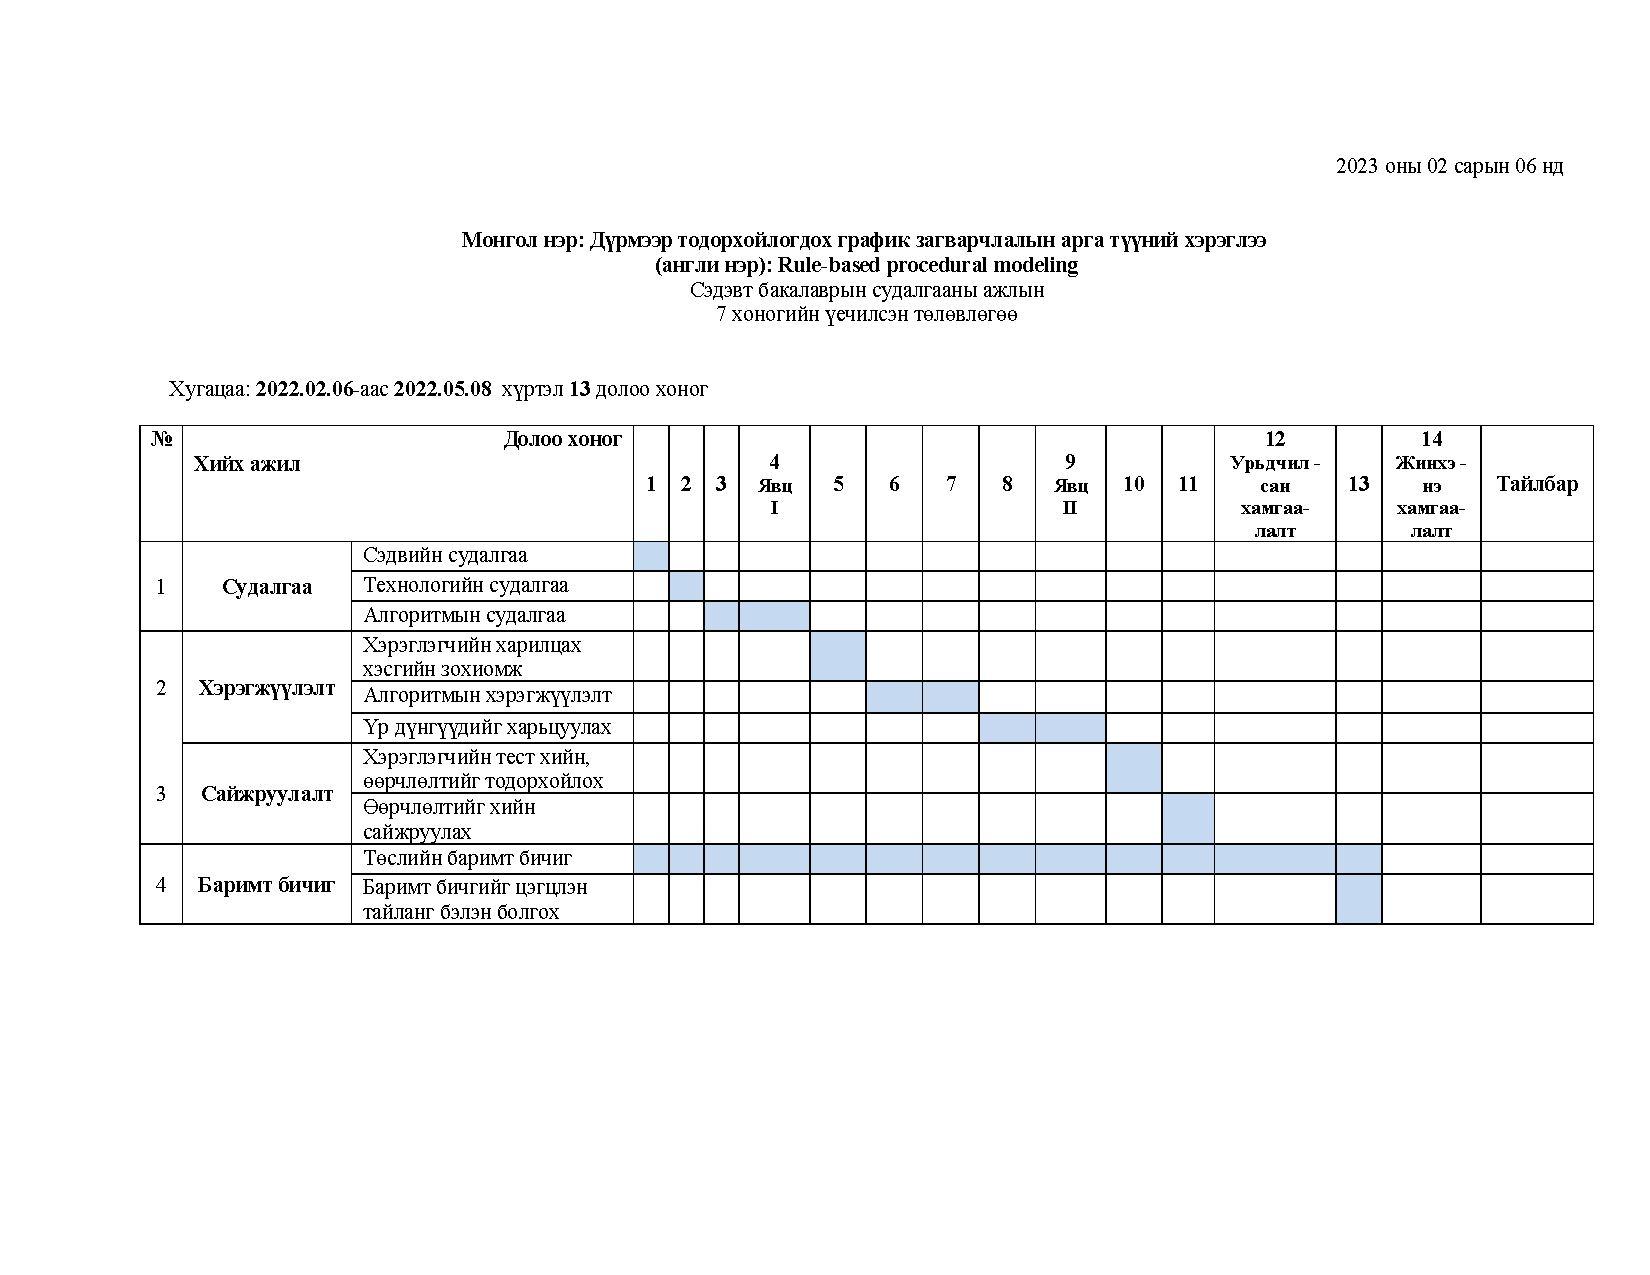
\includegraphics[angle=90,height=\textheight]{./images/plan.pdf}
	\caption{Ажлын төлөвлөгөө}
	\label{fig:WorkPlan}
\end{figure}

\end{document}
